\documentclass[tikz,border=4pt]{standalone}
\usepackage{amsmath,amssymb}
% Grupo Nostradamus - lenguaje visual TikZ
\definecolor{nostranavy}{HTML}{061426}
\definecolor{nostrateal}{HTML}{078C95}
\definecolor{nostracyan}{HTML}{65DCE5}
\definecolor{nostragold}{HTML}{F5C542}
\newcommand{\sen}{\operatorname{sen}}

\begin{document}
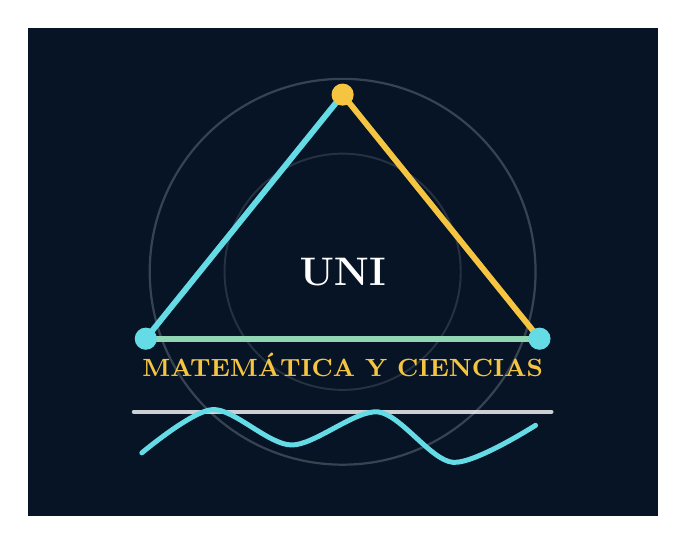
\begin{tikzpicture}[line cap=round,line join=round]
\fill[nostranavy] (-4,-3.1) rectangle (4,3.1);
\draw[white,opacity=.20,line width=.8pt] (0,0) circle (2.45);
\draw[white,opacity=.13,line width=.7pt] (0,0) circle (1.50);
\coordinate (A) at (-2.5,-.85); \coordinate (B) at (0,2.25); \coordinate (C) at (2.5,-.85);
\draw[nostracyan,line width=2.1pt] (A)--(B);
\draw[nostragold,line width=2.1pt] (B)--(C);
\draw[nostracyan!70!nostragold,line width=2.1pt] (C)--(A);
\fill[nostracyan] (A) circle (4pt); \fill[nostragold] (B) circle (4pt); \fill[nostracyan] (C) circle (4pt);
\node[white,font=\bfseries\Large] at (0,0) {UNI};
\node[nostragold,font=\bfseries\small] at (0,-1.18) {MATEM\'ATICA Y CIENCIAS};
\draw[white,opacity=.80,line width=1.6pt] (-2.65,-1.78)--(2.65,-1.78);
\draw[nostracyan,line width=1.8pt] plot[smooth] coordinates {(-2.55,-2.30) (-1.65,-1.75) (-.65,-2.20) (.45,-1.78) (1.40,-2.42) (2.45,-1.95)};
\end{tikzpicture}
\end{document}
